\subsection{}
\begin{enumerate}
 \item $a\leq a$. 
 \item $a\leq b, b\leq a \implies a \cong b$. 
 \item $a\leq b, b\leq c\implies a\leq c$. 
\end{enumerate}
のうち,(i), (iii) については容易である.(ii) について,有限グラフならば成り立ち無限グラフについては反例があることを示す.

$G$, $H$ を有限グラフとし,互いにマイナーであるとする.マイナーは縮約と部分グラフをとる操作と同型写像で得られ,
これらは頂点と辺の個数を増加させない操作である.有限グラフであることを使って元の個数を比べることで,
$|G|+\|G\| = |H| + \|H\|$ であり,頂点・辺が同一の縮約・部分グラフ・同型でうつりあう.頂点,辺の個数を変えない
縮約・部分グラフは自分自身に限られるから示された.

無限グラフについて,(ii) がこわれる.反例を作る.

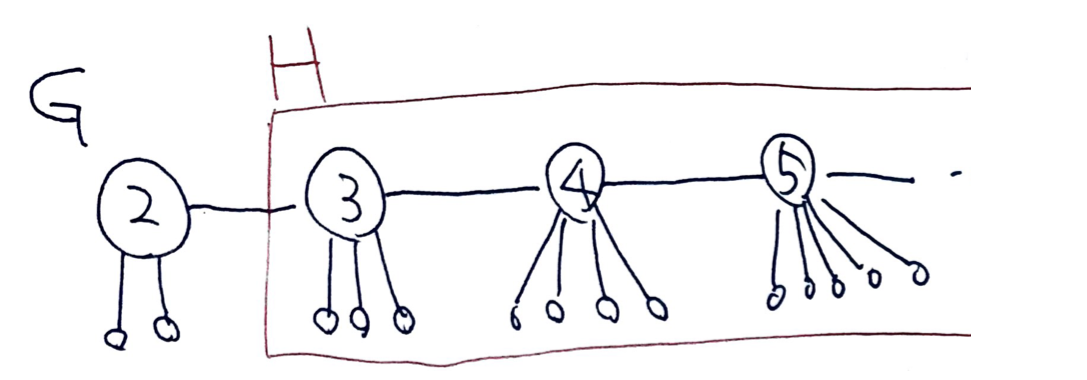
\includegraphics[width=\linewidth]{chap1/1_33.png}

$n\geq 2$ を半直線上に並べつつ,$n$ に隣接点を $n$ 個ずつ追加して図のようなグラフを作る.
$H$ は $G$ の部分グラフである.
$H$ から $3,4,5,\ldots$ の隣接点をひとつずつ削除すると $G$ と同型な部分グラフが得られる.
よって $G, H$ は互いにマイナーである.一方,$G$ と $H$ は同型でない.例えば $G$ には次数 $3$ の頂点が存在し,
$H$ には次数 $3$ の頂点が存在しないことから確かめられる.
反例が作れた.